\documentclass{article}
\usepackage[utf8]{inputenc}
\usepackage{enumerate}
\usepackage{amsmath}
\usepackage{amssymb}
\usepackage{amsfonts}
\usepackage{amstext}
\usepackage{amsthm}
\usepackage{mathtools}
\usepackage{tikz}
\usepackage{amsmath}
\usepackage{cancel}
\DeclarePairedDelimiter{\ceil}{\lceil}{\rceil}
\title{Calculus III Review Sheet 1 Practice}
\author{Eddie Ozuna and Tyler Franklin}

\begin{document}
\maketitle
\section{Dot Products}
\begin{enumerate}[a.]
	\item \textbf{What is the geometric significance of the dot product? }
	      \\
	      Two vectors are orthogonal(Perpendicular) if and only if the result of the dot product is equal to zero.\\\\
	      $\vec{u} = <u_{1},u_{2},u_{3}>\hspace{.4cm}\vec{v} = <v_{1},v_{2},v_{3}>$\\
	      \\
	      Reminder in how to perform the dot product:\\
	      \\
	      $\vec{u} \cdot \vec{v} = (u_{1} \cdot v_{1}) + (u_{2} \cdot v_{2}) + (u_{3} \cdot v_{3}) $\\
	      \\
	      Another Approach in how to perform the dot product:\\
	      \\
	      $\vec{u} \cdot \vec{v} =  \mid\vec{u}\mid\mid\vec{v}\mid\cos(\theta)$\\
	      \\
	      $\mid\vec{u}\mid = \sqrt{u_{1}\hspace{.001cm}^{2}+u_{2}\hspace{.001cm}^{2}+u_{3}\hspace{.001cm}^{2}}$\\
	      \\
	      $\mid\vec{v}\mid = \sqrt{v_{1}\hspace{.001cm}^{2}+v_{2}\hspace{.001cm}^{2}+v_{3}\hspace{.001cm}^{2}}$\\
	      \\
	      $\theta$ = The angle between the two vectors $\vec{u}$ and $\vec{v}$
\end{enumerate}
\begin{enumerate}[b.]
	\item \textbf{Why does the dot product have such geometric significance? Can you prove it? Hint: Remember the Pythagorean Theorem and its degeneration into the Law of Cosines. Can
	      you draw a picture to describe the scenario? }\\
	\\
	Given the definition above, where $\theta$ is the angle between $\vec{u}$ and $\vec{v}$, we can be certain that a result of $0$ means $\cos(\theta)=0$ which in turn means $\theta=\frac{\pi}{2}$ or $\theta=\frac{3\pi}{2}$ i.e. either a 90$^{\circ}$ or 270$^{\circ}$ perpendicular angle.\\
		
	Derivation: Law of Cosine\\
	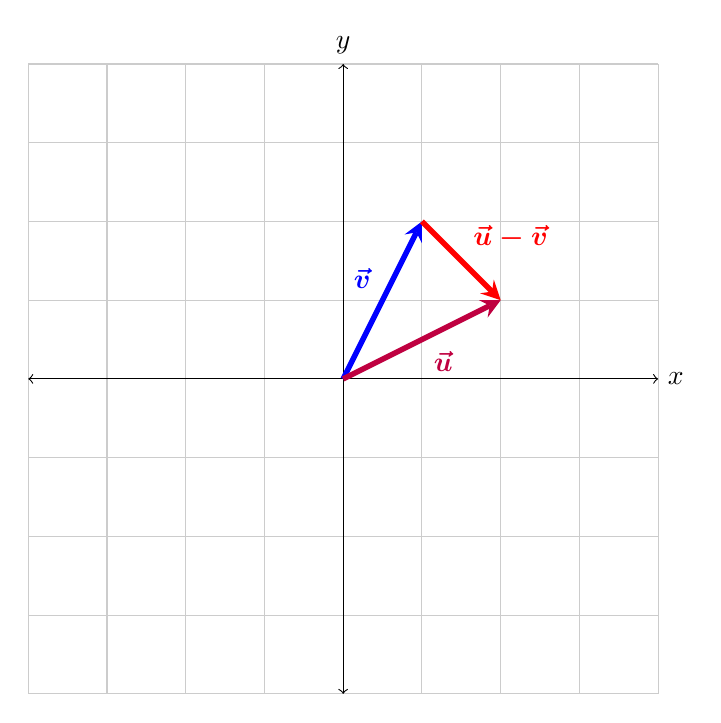
\begin{tikzpicture}
		\draw[thin,gray!40] (-4,-4) grid (4,4);
		\draw[<->] (-4,0)--(4,0) node[right]{$x$};
		\draw[<->] (0,-4)--(0,4) node[above]{$y$};
		\draw[line width=2pt,blue,-stealth](0,0)--(1,2) coordinate (VecV) node[midway,auto]{$\boldsymbol{\vec{v}}$};
		\draw[line width=2pt,purple,-stealth](0,0)--(2,1) coordinate (VecU) node[midway,auto,swap]{$\boldsymbol{\vec{u}}$};
		\draw[line width=2pt,red,-stealth](1,2)--(2,1) node[midway,auto]{$\boldsymbol{\vec{u}-\vec{v}}$};
		  
	\end{tikzpicture}\\
	\\
	$\mid\vec{u}-\vec{v}\mid^{2} = \mid\vec{u}\mid^{2} + \mid\vec{v}\mid^{2}-\hspace{.1cm}2\mid\vec{u}\mid\cdot\mid\vec{v}\mid\cos(\theta)$\\
	\\
	$\cancel{\mid\vec{u}\mid^{2}}-\hspace{.1cm}2\vec{v}\cdot\vec{u}\hspace{.1cm}+\cancel{\mid\vec{v}\mid^{2}}=\cancel{\mid\vec{u}\mid^{2}} + \cancel{\mid\vec{v}\mid^{2}}-2\mid\vec{u}\mid\cdot\mid\vec{v}\mid\cos(\theta)$\\
	\\
	$\cancel{-2}\vec{v}\cdot\vec{u} = \cancel{-2}\mid\vec{u}\mid\cdot\mid\vec{v}\mid\cos(\theta)$\\
	\\
	$\vec{v}\cdot\vec{u} = \mid\vec{u}\mid\cdot\mid\vec{v}\mid\cos(\theta)$\\
\end{enumerate}
\section{Cross Products}
\begin{enumerate}[a.]
	\item \textbf{What is the geometric significance of the cross product of two vectors?}\\
	      \\
	      It will always yield a new vector that is orthogonal(perpendicular) to the two vectors you took the cross product.\\
	      \\
	      
	      $\hspace{1cm}\hat{i}\hspace{.4cm}\hat{j}\hspace{.3cm}\hat{k}\hspace{2cm}\hat{i}\hspace{.4cm}\hat{j}\hspace{.3cm}\hat{k}\\\vec{u} = <u_{1},u_{2},u_{3}>\hspace{.4cm}\vec{v} = <v_{1},v_{2},v_{3}>$\\
	      \\
	      Reminder in how to perform the cross product:\\
	      \\
	      $\vec{u}\times\vec{v}=\begin{vmatrix}
	      \hat{i}&\hat{j}&\hat{k}\\
	      u_{1}&u_{2}&u_{3}\\
	      v_{1}&v_{2}&v_{3}\\
	\end{vmatrix}=\hat{i}
	\begin{vmatrix}
		u_{2} & u_{3} \\
		v_{2} & v_{3} \\
	\end{vmatrix}-\hat{j}\begin{vmatrix}
	u_{1}&u_{3}\\
	v_{1}&v_{3}\\
	\end{vmatrix}+\hat{k}\begin{vmatrix}
	u_{1}&u_{2}\\
	v_{1}&v_{2}\\
	\end{vmatrix}\\
	=\hat{i}(u_{2}v_{3}-u_{3}v_{2})-\hat{j}(u_{1}v_{3}-u_{3}v_{1})+\hat{k}(u_{1}v_{2}-u_{2}v_{1})$\\
	\\
	Another Approach in how to perform the cross product:\\
	\\
	$\vec{u} \times \vec{v} =  \mid\vec{u}\mid\mid\vec{v}\mid\sin(\theta)$\\
	\\
	$\mid\vec{u}\mid = \sqrt{u_{1}\hspace{.001cm}^{2}+u_{2}\hspace{.001cm}^{2}+u_{3}\hspace{.001cm}^{2}}$\\
	\\
	$\mid\vec{v}\mid = \sqrt{v_{1}\hspace{.001cm}^{2}+v_{2}\hspace{.001cm}^{2}+v_{3}\hspace{.001cm}^{2}}$\\
	\\
	$\theta$ = The angle between the two vectors $\vec{u}$ and $\vec{v}$
\end{enumerate}
\begin{enumerate}[b.]
	\item \textbf{Why does the cross product have such geometric significance?}\\
	      \\
\end{enumerate}
\section{Orthagonality}
\begin{enumerate}[a.]
	\item \textbf{Prove that the cross product $\vec{u} \times \vec{v}$ of two vectors $\vec{u}$ and $\vec{v}$ is actually orthogonal(perpendicular) to each of $\vec{u}$ and $\vec{v}$ simultaneously.}\\
	      \\
	      
	      $\hspace{1cm}\hat{i}\hspace{.4cm}\hat{j}\hspace{.3cm}\hat{k}\hspace{2cm}\hat{i}\hspace{.4cm}\hat{j}\hspace{.3cm}\hat{k}\\\vec{u} = <u_{1},u_{2},u_{3}>\hspace{.4cm}\vec{v} = <v_{1},v_{2},v_{3}>$\\
	      \\
	      \textbf{Step 1.} Take the cross product of $\vec{u}$ and $\vec{v}$\\
	      \\
	      $\vec{u}\times\vec{v}=\begin{vmatrix}
	      \hat{i}&\hat{j}&\hat{k}\\
	      u_{1}&u_{2}&u_{3}\\
	      v_{1}&v_{2}&v_{3}\\
	\end{vmatrix}=\hat{i}
	\begin{vmatrix}
		u_{2} & u_{3} \\
		v_{2} & v_{3} \\
	\end{vmatrix}-\hat{j}\begin{vmatrix}
	u_{1}&u_{3}\\
	v_{1}&v_{3}\\
	\end{vmatrix}+\hat{k}\begin{vmatrix}
	u_{1}&u_{2}\\
	v_{1}&v_{2}\\
	\end{vmatrix}\\
	=\hat{i}(u_{2}v_{3}-u_{3}v_{2})-\hat{j}(u_{1}v_{3}-u_{3}v_{1})+\hat{k}(u_{1}v_{2}-u_{2}v_{1})$\\
	\\
	Let $\vec{w}$ be equal to the result of the cross product of $\vec{u}$ and $\vec{v}$:\\
	$\vec{w} = \hat{i}(u_{2}v_{3}-u_{3}v_{2})-\hat{j}(u_{1}v_{3}-u_{3}v_{1})+\hat{k}(u_{1}v_{2}-u_{2}v_{1})$\\
	\\
	\textbf{Step 2.} From our previous knowledge we know that if the result of the dot product is zero the vectors are orthogonal(perpendicular). With that being said let perform the dot products of vector $\vec{u}$ with $\vec{w}$ and $\vec{v}$ with $\vec{w}$.\\
	\\
	$\vec{w} = <(u_{2}v_{3}-u_{3}v_{2}),-(u_{1}v_{3}-u_{3}v_{1}),(u_{1}v_{2}-u_{2}v_{1})>$\\
	\\
	$\vec{u}\cdot\vec{w}=u_{1}(u_{2}v_{3}-u_{3}v_{2})-u_{2}(u_{1}v_{3}-u_{3}v_{1})+u_{3}(u_{1}v_{2}-u_{2}v_{1})\\=u_{1}u_{2}v_{3}-u_{1}v_{2}u_{3}-u_{1}u_{2}v_{3}+v_{1}u_{2}u_{3}+u_{1}u_{3}v_{2}-v_{1}u_{2}u_{3}=0$\\
	\\ 
	$\vec{v}\cdot\vec{w}=v_{1}(u_{2}v_{3}-u_{3}v_{2})-v_{2}(u_{1}v_{3}-u_{3}v_{1})+v_{3}(u_{1}v_{2}-u_{2}v_{1})\\=v_{1}u_{2}v_{3}-v_{1}v_{2}u_{3}-u_{1}v_{2}v_{3}+v_{1}v_{2}u_{3}+u_{1}v_{2}v_{3}-v_{1}u_{2}v_{3}=0$\\
	\\
	Proven Both yield a result of zero which state they are orthogonal(perpendicular) simultaneously.
\end{enumerate}
\begin{enumerate}[b.]
	\item\textbf{Find a vector that is orthogonal(perpendicular) to each of the vectors $e_{1}:= \left(\!
	      \begin{array}{c}
	      	1 \\
	      	0 \\
	      	0 
	      \end{array}
	      \!\right)$ and $e_{2}:=\left(\!
	      \begin{array}{c}
	      	0 \\
	      	1 \\
	      	0 
	      \end{array}
	      \!\right)$}
	\\
	\\
	From previous knowledge we know that taking the cross product of two vectors yield us a new vector that is orthogonal(perpendicular) to does two vectors. With that being said let perform the cross products of $e_{1}$ with $e_{2}$.
	\\\\
	$e_{1}=<1,0,0>\hspace{.4cm}e_{2}=<0,1,0>$\\
	\\
	$e_{1} \times e_{2}=\begin{vmatrix}
	\hat{i}&\hat{j}&\hat{k}\\
	1&0&0\\
	0&1&0\\
	\end{vmatrix}=\hat{i}\begin{vmatrix}
	0&0\\
	1&0\\
	\end{vmatrix}-\hat{j}\begin{vmatrix}
	1&0\\
	0&0\\
	\end{vmatrix}+\hat{k}\begin{vmatrix}
	1&0\\
	0&1\\
	\end{vmatrix}=0\hat{i}-0\hat{j}+1\hat{k}$\\
	\\
	Let $e_{3}$ equal the result of the cross  products of $e_{1}$ with $e_{2}$.\\
	\\
	$e_{3}=<0,0,1>$
\end{enumerate}
\begin{enumerate}[c.]
	\item\textbf{Prove that your vector is actually perpendicular to each of $e_{1}$ and $e_{2}$ simultaneously}\\
	\\
	From our previous knowledge we know that if the result of the dot product is zero the vectors are orthogonal(perpendicular). With that being said let perform the dot products of vector $e_{1}$ with $e_{3}$ and $e_{2}$ with $e_{3}$.\\
	\\
	$e_{1}=<1,0,0>\hspace{.4cm}e_{2}=<0,1,0>\hspace{.4cm}e_{3}=<0,0,1>$\\
	\\
	$e_{1} \cdot e_{3}=(1 \cdot 0) + (0 \cdot 0 ) + (0 \cdot 1) = 0$\\
	\\
	$e_{2} \cdot e_{3}=(0 \cdot 0) + (1 \cdot 0 ) + (0 \cdot 1) = 0$\\
	\\
	Proven Both yield a result of zero which state they are orthogonal(perpendicular)
\end{enumerate}
\section{Determinants}
\begin{enumerate}[a.]
	\item\textbf{The volume of the parallelopiped (three-dimensional analogue of a parallelo-
	      gram) spanned by three vectors $\vec{u}$, $\vec{v}$ and $\vec{w}$ is given by:}\\
	\\
	$(\vec{u}\times\vec{v})\cdot\vec{w}:=<\vec{u}\times\vec{v},\vec{w}>$\\
	\\ This just mean take the cross product of $\vec{u}$ with $\vec{v}$ and then take the dot product of the result with $\vec{w}$. Both side mean the same thing just different notation for the dot product!\\
	\\
	\textbf{This is known as the triple product of $\vec{u}$, $\vec{v}$ and $\vec{w}$. Interestingly enough, this is a way of defining the determinant of a matrix. Given a matrix:}\\
	\\
	$M:=\begin{vmatrix}
	u_{1}&v_{1}&w_{1}\\
	u_{2}&v_{2}&w_{2}\\
	u_{3}&v_{3}&w_{3}\\
	\end{vmatrix}$\\
	\\
	\textbf{where we notice that the columns of the matrix are precisely the vectors $\vec{u}$, $\vec{v}$ and $\vec{w}$. we can actually define the determinant of the matrix M via:}\\
	\\
	$det(M ) := <\vec{u}\times\vec{v},\vec{w}>$\\
	\\
	\textbf{Prove that these two definitions yield the same thing! The determinant of a
		matrix is said to encode the amount that the unit parallelopiped is scaled upon
		applying the linear transformation of space represented by the matrix.}\\
	\\
	To prove this we just need to take the determinant of M which is the left side of the equation and them evaluate the right side of the question which just mean take the cross product of $\vec{u}$ with $\vec{v}$ and then take the dot product of the result with $\vec{w}$.\\
	\\
	Left side of the equation:\\
	\\
	$det(M ) := \begin{vmatrix}
	u_{1}&v_{1}&w_{1}\\
	u_{2}&v_{2}&w_{2}\\
	u_{3}&v_{3}&w_{3}\\
	\end{vmatrix}=u_{1}\begin{vmatrix}
	v_{2}&w_{2}\\
	v_{3}&w_{3}\\
	\end{vmatrix}-v_{1}\begin{vmatrix}
	u_{2}&w_{2}\\
	u_{3}&w_{3}\\
	\end{vmatrix}+w_{1}\begin{vmatrix}
	u_{2}&v_{2}\\
	u_{3}&v_{3}\\
	\end{vmatrix}\\\\:=u_{1}(v_{2}w_{3} - w_{2}v_{3}) - v_{1}(u_{2}w_{3}-w_{2}u_{3})+w_{1}(u_{2}v_{3}-v_{2}u_{3})\\:=u_{1}v_{2}w_{3} - u_{1}w_{2}v_{3}-v_{1}u_{2}w_{3}+v_{1}w_{2}u_{3}+w_{1}u_{2}v_{3}-w_{1}v_{2}u_{3}$\\
	\\
	\\
	Right side of the equation:\\
	\\
	$<\vec{u}\times\vec{v},\vec{w}>$\\
	\\
	$\vec{u}\times\vec{v}=\begin{vmatrix}
	\hat{i}&\hat{j}&\hat{k}\\
	u_{1}&u_{2}&u_{3}\\
	v_{1}&v_{2}&v_{3}\\
	\end{vmatrix}=\hat{i}
	\begin{vmatrix}
		u_{2} & u_{3} \\
		v_{2} & v_{3} \\
	\end{vmatrix}-\hat{j}\begin{vmatrix}
	u_{1}&u_{3}\\
	v_{1}&v_{3}\\
	\end{vmatrix}+\hat{k}\begin{vmatrix}
	u_{1}&u_{2}\\
	v_{1}&v_{2}\\
	\end{vmatrix}\\
	=\hat{i}(u_{2}v_{3}-u_{3}v_{2})-\hat{j}(u_{1}v_{3}-u_{3}v_{1})+\hat{k}(u_{1}v_{2}-u_{2}v_{1})$\\
	\\
	$<\vec{u}\times\vec{v},\vec{w}> := w_{1}(u_{2}v_{3}-u_{3}v_{2})-w_{2}(u_{1}v_{3}-u_{3}v_{1})+w_{3}(u_{1}v_{2}-u_{2}v_{1})\\:=w_{1}u_{2}v_{3}-w_{1}u_{3}v_{2}-w_{2}u_{1}v_{3}+w_{2}u_{3}v_{1}+w_{3}u_{1}v_{2}-w_{3}u_{2}v_{1}$\\
	\\
	You can clearly see that they are equal to each other proven!
\end{enumerate}
\begin{enumerate}[b.]
	\item\textbf{Draw the result of applying this linear transformation to the unit parallelopiped spanned by the basis vectors $\vec{e_{1}}$ , $\vec{e_{2}}$ , and $\vec{e_{3}}$. The volume of the unit parallelop-iped is, of course, 1·1·1 = 1.}\\
	\\
\end{enumerate}
\begin{enumerate}[c.]
	\item\textbf{What is the volume of the new parallelopiped after
	      the linear transformation described by the matrix? Compute the determinant
	      of this matrix, and also the quantity and verify that they are equal, verifying that, at least in this case, the determi-nant of the matrix describing the linear transformation does in fact encode the change in volume of the unit parallelopiped under this transformation of space!}\\
	\\
	Just evaluate each one and check if the results are equal.\\
	1.)
	$M:=\left(\!
	\begin{array}{c}
		1 \hspace{.5cm} 2 \hspace{.5cm} 3 \\
		4 \hspace{.5cm} 5 \hspace{.5cm} 6 \\
		7 \hspace{.5cm} 8 \hspace{.5cm} 8 \\
	\end{array}
	\!\right)$\\
	\\  
	\\
	\\
	$det(M ) := \begin{vmatrix}
	1&2&3\\
	4&5&6\\
	7&8&8\\
	\end{vmatrix}:=1\begin{vmatrix}
	5&6\\
	8&8\\
	\end{vmatrix}-2\begin{vmatrix}
	4&6\\
	7&8\\
	\end{vmatrix}+3\begin{vmatrix}
	4&5\\
	7&8\\
	\end{vmatrix}\\:=1(5\cdot8-6\cdot8)-2(4\cdot8-6\cdot7)+3(4\cdot8-5\cdot7)\\:=-8+20-9:=3$\\
	\\
	2.)
	$\left<\vec{u}:=\left(\!
	\begin{array}{c}
		1 \\
		4 \\
		7 
	\end{array}
	\!\right)\times\vec{v}:=\left(\!
	\begin{array}{c}
		2 \\
		5 \\
		8 
	\end{array}
	\!\right),\vec{w}:=\left(\!
	\begin{array}{c}
		3 \\
		6 \\
		8 
	\end{array}
	\!\right)\right>$\\ 
	$\vec{u}\times\vec{v}=\begin{vmatrix}
	\hat{i}&\hat{j}&\hat{k}\\
	1&4&7\\
	2&5&8\\
	\end{vmatrix}=\hat{i}\begin{vmatrix}
	4&7\\
	5&8\\
	\end{vmatrix}-\hat{j}\begin{vmatrix}
	1&7\\
	2&8\\
	\end{vmatrix}+\hat{k}\begin{vmatrix}
	1&4\\
	2&5\\
	\end{vmatrix}\\ = \hat{i}(4 \cdot 8-7 \cdot5)-\hat{j}(1\cdot8-7\cdot2)+\hat{j}(1\cdot5-4\cdot2)\\=-3\hat{i}+6\hat{j}-3\hat{k}$\\
	\\
	$<\vec{u}\times\vec{v},\vec{w}>=(-3\cdot3)+(6\cdot6)+(-3\cdot8)=3 $\\
\end{enumerate}
\section{Spanning planes and normals}
\begin{enumerate}[a.]
	\item\textbf{Find a line passing through the point $\left(\!
	      \begin{array}{c}
	      	1 \\
	      	2 \\
	      	3 
	      \end{array}
	      \!\right)$ normal to the plane passing through $\left(\!
	      \begin{array}{c}
	      	2 \\
	      	3 \\
	      	4 
	      \end{array}
	      \!\right)$,$\left(\!
	      \begin{array}{c}
	      	5 \\
	      	6 \\
	      	7 
	      \end{array}
	      \!\right)$, and $\left(\!
	      \begin{array}{c}
	      	8 \\
	      	9 \\
	      	9 
	      \end{array}
	      \!\right)$ }\\
	\\
	\textbf{Step 1.} Find the equation of the plane passing through $\left(\!
	\begin{array}{c}
		2 \\
		3 \\
		4 
	\end{array}
	\!\right)$,$\left(\!
	\begin{array}{c}
		5 \\
		6 \\
		7 
	\end{array}
	\!\right)$, and $\left(\!
	\begin{array}{c}
		8 \\
		9 \\
		9 
	\end{array}
	\!\right)$\\
	\\
	Let $\vec{p}=<2,3,4>, \vec{q}=<5,6,7>,$ and $\vec{k}=<8,9,9>$\\
	\\
	Let $\vec{pq} = <5-2,6-3,7-4>=<3,3,3>$\\
	\\
	Let $\vec{pk} = <8-5,9-6,9-7>=<3,3,2>$\\
	\\
	Take the cross product of vectors $\vec{pq}$ with $\vec{pk}$\\
	\\
	$\vec{pq}\times\vec{pk}=\begin{vmatrix}
	\hat{i}&\hat{j}&\hat{k}\\
	3&3&3\\
	3&3&2\\
	\end{vmatrix}=\hat{i}\begin{vmatrix}
	3&3\\
	3&2\\
	\end{vmatrix}-\hat{j}\begin{vmatrix}
	3&3\\
	3&2\\
	\end{vmatrix}+\hat{k}\begin{vmatrix}
	3&3\\
	3&3\\
	\end{vmatrix}\\
	=\hat{i}(3 \cdot 2-3 \cdot3)-\hat{j}(3\cdot2-3\cdot3)+\hat{j}(3\cdot3-3\cdot3)
	\\=-3\hat{i}+3\hat{j}+0\hat{k}$\\
	\\
	General form of a equation of a plane a(x-$x_{0}$)+b(y-$y_{0}$)+c(z-$z_{0}$)=0\\
	\\
	$\vec{pq}\times\vec{pk}=<-3,3,0>$\\
	\\
	a = -3 , b = 3 , c = 0\\
	\\
	plane = -3(x-2)+3(y-3)+0(z-4)=0
	\\
	\\
	normal vector $\vec{n}=<-3,3,0>$ \\
	\\
	\\
	\textbf{Step 2.} Parameterized using the normal vector of the equation of the plane to get the equation of the lines using the point $<1,2,3>$\\
	\\
	x(t)=1-3t\\
	y(t)=2+3t\\
	z(t)=3+0t\\
	
\end{enumerate}
	
\section{3D Space}
\begin{enumerate}[a.]
    \item\textbf{ In how many ways can two lines intersect in three-dimensional space? Draw all of the ways and provide examples.} 
    
    Two lines can intersect once, intersect infinitely (i.e. overlapping), or never intersect (i.e. parallel or skew lines).
    
    \item\textbf{ In two-dimensional space, two lines with different slopes must intersect. In three-dimensional space, is this still true? If so, prove it. Else, provide an explicit counterexample.}
    
    It is not necessarily true in 3D space. Lines with different slopes could, where they might intersect given a certain 2D perspective, be separated in the 3rd dimension. For example, you could cross drumsticks in front of you, such that they were touching, or you could push/pull them apart slightly, such that they still crossed each other, but didn't touch.
    
    \item\textbf{ In how many ways can two planes intersect in three-dimensional space? Draw all of the ways and provide examples.} 
    
    Two planes can intersect once at a line, infinitely (i.e. overlapping), or not at all (i.e. such that their normals were parallel to one another).
\end{enumerate}
	  
\section{Conic sections}
\textbf{In two-dimensional space, all quadric curves, i.e. conic sections, are described/parameterized by a “master equation”:}

\[Ax^{2} + Bxy + Cy^2 + Dx + Ey + F = 0\]

\textbf{Convince yourself that every conic section arises from choosing different values of the coefficients $A-F$.}\newline

We can see it is true by the forms of known quadric curves: \newline

\hspace{1cm} \textbf{Circle:} $A=1, B=0, C=1, D=0, E=0, F=-1$
    \[x^2 + y^2 - 1 = 0\]

\hspace{1cm} \textbf{Ellipse:} $A=\frac{1}{2}, B=0, C=\frac{1}{2}, D=0, E=0, F=-1$
    \[\frac{x^2}{2} + \frac{y^2}{2} - 1 = 0\]

\hspace{1cm} \textbf{Parabola:} $A=0, B=0, C=-1, D=4, E=0, F=0$
    \[4x - y^2 = 0\]

\hspace{1cm} \textbf{Hyperbola:} $A=\frac{1}{2}, B=0, C=-\frac{1}{2}, D=0, E=0, F=-1$ 
    \[\frac{x^2}{a^2} - \frac{y^2}{b^2} - 1 = 0\]

Each of these are created by changing coefficients $A-F$ of the master equation. 

\section{Quadrics}

\textbf{In three-dimensional space, we have the quadric surfaces described/parameterized by the “master equation”:}
\[Ax^2 + By^2 + Cz^2 + Dxy + Exz + Fyz + Gx + Hy + Iz + J = 0\]

\begin{enumerate}[a.]
    \item\textbf{Convince yourself that every quadric surface arises from choosing different values of the coefficients $A−J$.}
    
    We illustrate this below.
    
    \item\textbf{Are the conic sections a special case of the quadric surfaces? Why or why not?}
    
    Yes, quadric surfaces are the generalization of conic sections, which is to say when any quadric surface intersects a coordinate plane, the trace is a conic section.
    
    \item\textbf{Find the coefficients that describe a sphere, a paraboloid, a hyperboloid, etc.}
    
\hspace{1cm} \textbf{Sphere:} $A=1, B=1, C=1, D=0, E=0, F=0, G=0, H=0, I=0, K=-1$
    \[x^2 + y^2 + z^2 - 1 = 0\]

\hspace{1cm} \textbf{Paraboloid:} $A=\frac{1}{2}, B=-\frac{1}{2}, C=0, D=4, E=0, F=0, G=0, H=0, I=-1, J=0, K=0$
    \[\frac{x^2}{2} - \frac{y^2}{2} - z = 0\]

\hspace{1cm} \textbf{Hyperboloid:} $A=\frac{1}{a^2}, B=\frac{1}{b^2}, C=-\frac{1}{c^2}, D=0, E=0, F=0, G=0, H=0, I=0, J=0, K=-1$ 
    \[\frac{x^2}{a^2} + \frac{y^2}{b^2} - \frac{z^2}{c^2} - 1 = 0\]

\end{enumerate}

\section{Tangent and normal vectors}
\textbf{The twisted cubic curve is parameterized by a single parameter t via:} 
\[
t\mapsto\left(\begin{array}{c}x(t) = t  y(t)=t^{2}   z(t)=t^{3}\end{array} \right)
\]

\textbf{Find the parameterization of the tangent vector to the twisted cubic curve. Use your parameterization of the tangent vector to find a vector perpendicular to the twisted cubic curve at the point $(1,1,1)$ on the curve.}\newline

Let $c(t)=\left(x(t) = t, y(t)=t^{2}, z(t)=t^{3}\right)$ \newline

\textbf{Step 1.} Take the derivative of the components of c(t)

\[ \frac{dc}{dt}=\left(x(t) = 1, y(t)= 2t, z(t)=3t^{2}\right) \]

\textbf{Step 2.} Use $\frac{dc}{dt}$ to get the tangent vector at $(1,1,1)$

\[\frac{dc}{dt}(1, 1, 1) = (1,2,3)\]

\textbf{Step 3.} To get a normal to the surface at this point, we need a vector that's normal to the tangent we just computed: $(1,2,3)$. That is...

\[(1,2,3)\cdot\vec{v}=0\]
\[(1,2,3)\cdot(v_1,v_2,v_3)=0\]
\[(1\cdot v_1)+(2\cdot v_2)+(3 \cdot v_3) = 0\]

At this point we just pick values for $v_1, v_2, v_3$ which make the equation equal 0. For example, $(2, -1, 0)$ is a viable answer. We can check...

\[\vec{v} = (2, -1, 0)\]
\[(1,2,3)\cdot(2, -1, 0)=0\]
\[(1\cdot2)+(2\cdot-1)+(3\cdot0)=0\]
\[2-2+0=0\]

\section{Conic Sections}
\textbf{Find two surfaces whose intersection is the curve (ellipse) described by the equation:}
    
    \[\frac{x^2}{1^2}+\frac{y^2}{2^2}=1^2\]
    
    \textbf{There is a cheap answer; try to find a non-cheap answer! More specifically, see if you can figure out the equation of the plane whose intersection with the cone defined by the equation}
    
    \[x^2+y^2=z^2\]
    
    \textbf{is the ellipse described above. More ambitiously, can you find the plane whose intersection with this cone gives an arbitrary conic section?!}
    
    This is the illustrative example of conic sections. Intersecting the cone with a plane can provide an arbitrary ellipse which varies depending on the plane's orientation.
    
\section{Singularities}
\begin{enumerate}
    \item\textbf{At which point will the tangent plane to the cone described by}
    \[xy = z^2\]
    \textbf{be ill-defined?}
    
    At origin, $(0,0,0)$.
    
    \item\textbf{Can you explain why?}
    
    At the origin, the value is indeterminate because that point on the surface is a singularity -- i.e. it is "sharp."
    
    \item\textbf{What does this surface look like?}
    
    It's an infinite elliptic cone.
\end{enumerate}

\section{Directional derivative}
\textbf{Consider the surface that is the graph of the function $f(x,y):=x^3+x-y^5$. Calculate the directional derivative of the function $f(x, y) := x^2+y^2$ at the point $e_1 := (1,0)$ in the direction of the (unit) vector parallel to $e_2 := (0,1)$ using the limit definition and verify that it agrees with the directional derivative of $f(x, y)$ at the point $e_1$ in the direction of the (unit) vector $e_1$.}

\textbf{Step 1.} Calculate the directional derivative using the limit definition

\begin{equation}
\begin{split}
D_{u}f(\vec{p})& =\lim_{h \to 0} \frac{f(\vec{p}+h\cdot\vec{u})-f(\vec{p})}{h}\\
D_{u}f(1,0)& =\lim_{h \to 0} \frac{f(<1,0>+h\cdot<1,0>)-f(1,0)}{h}\\
& =\lim_{h \to 0} \frac{f(<1,0>+<h,0>)-f(1,0)}{h}\\
& =\lim_{h \to 0} \frac{f(<1+h,0+0>)-f(1,0)}{h}\\
& =\lim_{h \to 0} \frac{(1+h)^{2}+0^{2}-(1^{2}+0^{2})}{h}\\
& =\lim_{h \to 0} \frac{1+2h+h^{2}-1}{h}\\
& =\lim_{h \to 0} \frac{2h+h^{2}}{h}\\
& =\lim_{h \to 0} \frac{h(2+h)}{h}\\
& =\lim_{h \to 0} (2+h)\\
& =2
\end{split}
\end{equation}

	\textbf{Step 2.} Calculate the the product of the gradient $\nabla f(x,y)$ and $e_2$:
	\[\nabla f(x,y)=(2x,2y)\]
	\[\nabla f(0,1)=(2(0),2(1)) = (0,2)\]
	\[(0,2)\cdot(0,1)=(0\cdot0)+(2\cdot1)=2\]

\section{Unit sphere normals}
    \textbf{Find the normal vector to the surface defined by the equation $x^{2} + y^{2} + z^{2} =1^{2}$ at the point $(0,0,1)$ and use this normal vector to find the equation of the plane tangent to the surface at this point.}
\begin{enumerate}[a.]
    \item The first is a trick question. We can tell immediately that this is a unit sphere (i.e. $R=1$) so at the point $(0,0,1)$ a valid normal vector is... $(0,0,1)$ or some linear combination thereof, such as $(0,0,2)$.
    \item To find the tangent plane, we must use the general form of a equation of a plane: 
    \[a(x-x_{0})+b(y-y_{0})+c(z-z_{0})=0\]
	However since we know $a$ and $b$ will be multiples of 0, and $c$ a multiple of 1:
	\[(0)(x-(0))+(0)(y-(0))+(1)(z-(1))=0\]
	\[z-1=0\]
\end{enumerate}

\section{Gradient concept}

\textbf{Why is the direction of the gradient of a function at a point the direction along
which the value of the function will ascend most quickly? Why is the negative
of the gradient of a function at a point the direction along which the value of
the function will descend most quickly?}\newline

The answer to both questions is the nature of the gradient, as its speed/angle of descent is provided by the dot product. That is, if you project $\nabla f$ along any direction $\vec{v}$ \textit{other} than $\nabla f$ via the dot product...
\[\mid\vec{\nabla f}\mid\mid\vec{v}\mid\cos(\theta)\]
...by definition you will find that the maximum value is attained when $\cos(\theta)=1$, i.e. when $\theta=0$, which means $\vec{v}$ and $\nabla f$ are equal.
    

\section{Extrema}
\textbf{Find all extrema of the function $f(x,y) := 3x^{2}y+y^{3}-2x^{2}-2y^{2}+3$. In what direction from $(0,0,3)$ should we travel to ascend most quickly? descend most quickly? How do you know?}

\begin{enumerate}[a.]
    \item First, we take partial derivatives with respect to x and y.
    \[F_x=6xy-4x\]
    \[F_y=3x^{2}+3y^{2}-4y\]
    \item Next, use the results to take 2nd partial derivatives with respect to x-by-x and y-by-y, then x-by-y and y-by-x.
    \[F_{xx}=6y-4\]
    \[F_{yy}=6y-4\]
    \[F_{xy}=6\]
    \[F_{yx}=6x\]
    \item To find critical points, solve $F_x=0$ and $F_y=0$. We do this by solving one, then plugging into the other. So, starting with $F_x=0$
    \[6xy-4x=0\]
    We can see right away that $x=0$ is one solution, however also:
	\[6y=4\]
	\[y=\frac{2}{3}\]
	Next we plug the solutions above ($x=0$ and $y=\frac{2}{3}$) into $F_y=0$
	\[3x^{2}+3y^{2}-4y=0\]
	Starting with the simplest option, $x=0$, we get
	\[3(0)^{2}+3y^{2}-4y=0\]
	\[y(3y-4)=0\]
	Which tells us that, if $x=0$, then either $y=0$ or $y=\frac{4}{3}$. Next we check our other possibility: $y=\frac{2}{3}$
	\[3x^{2}+3\left(\frac{2}{3}\right)^{2}-4\left(\frac{2}{3}\right)=0\]
	\[3x^2+(\frac{4}{3})-\frac{8}{3}=0\]
	\[3x^2=\frac{4}{3}\]
	\[x=\sqrt{\frac{4}{9}}\]
	\[x=\pm\frac{2}{3}\]
	So our critical points are $(0,0)$, $\left(0,\frac{4}{3}\right)$, $\left(\frac{2}{3},\frac{2}{3}\right)$ and $\left(-\frac{2}{3},\frac{2}{3}\right)$.
	
	\item Finally, to determine whether the critical points are maximum, minimum, or saddle points, we can use the second partial derivative test:
	
	\begin{equation}
	    \begin{split}
	        D(x,y)&= \begin{vmatrix} F_{xx} & F_{xy} \\ F_{yx} & F_{yy} \end{vmatrix}\\
	        &=\begin{vmatrix}6y-4&6x\\6x&6y-4\end{vmatrix}
	    \end{split}
	\end{equation}
	
	Recall that $D(x,y)<0$ indicates a saddle point, $D(x,y)>0$ indicates either minimum or maximum, where we have to plug $F_{xx}$ to check which one, where $F_{xx}>0 \Rightarrow$ min and $F_{xx}<0\Rightarrow$ max, and  $D(x,y)=0$ indicates $undefined$.
	
	\begin{equation}
    \begin{split}
        D\left(0,0\right)&=\begin{vmatrix}6(0)-4&6(0)\\6(0)&6(0)-4\end{vmatrix} \\
    	&=\begin{vmatrix}-4&0\\0&-4\end{vmatrix}\\
    	&=(-4\cdot-4)-(0\cdot0)\\
    	&=16-0\\
    	&=16
    \end{split}
	\end{equation}
	
	\[F_{xx}(0,0)=6(0)-4=-4\]
	
	\[\therefore \left(0,0\right) = max\]
	
	\begin{equation}
    \begin{split}
        D\left(0,\frac{4}{3}\right)&=\begin{vmatrix}6(\frac{4}{3})-4&6(0)\\6(0)&6(\frac{4}{3})-4\end{vmatrix} \\
    	&=\begin{vmatrix}4&0\\0&4\end{vmatrix}\\
    	&=(4\cdot4)-(0\cdot0)\\
    	&=16-0\\
    	&=16
    \end{split}
	\end{equation}
	
	\[F_{xx}\left(0,\frac{4}{3}\right)=6\left(\frac{4}{3}\right)-4=4\]
	
	\[\therefore \left(0,0\right) = min\]
	
	\begin{equation}
    \begin{split}
        D\left(\frac{2}{3},\frac{2}{3}\right)&=\begin{vmatrix}6(\frac{2}{3})-4&6(\frac{2}{3})\\6(\frac{2}{3})&6(\frac{2}{3})-4\end{vmatrix} \\
    	&=\begin{vmatrix}2(2)-4&2(2)\\2(2)&2(2)-4\end{vmatrix}\\
    	&=\begin{vmatrix}0&4\\4&0\end{vmatrix}\\
    	&=(0\cdot0)-(4\cdot4)\\
    	&=0-16\\
    	&=-16
    \end{split}
	\end{equation}
	
	\[\therefore \left(\frac{2}{3},\frac{2}{3}\right) = saddle\]
	
	\begin{equation}
    \begin{split}
        D\left(\frac{2}{3},-\frac{2}{3}\right)&=\begin{vmatrix}6(\frac{2}{3})-4&6(-\frac{2}{3})\\6(-\frac{2}{3})&6(\frac{2}{3})-4\end{vmatrix} \\
    	&=\begin{vmatrix}2(2)-4&2(-2)\\2(-2)&2(2)-4\end{vmatrix}\\
    	&=\begin{vmatrix}0&-4\\-4&0\end{vmatrix}\\
    	&=(0\cdot0)-(-4\cdot-4)\\
    	&=0-16\\
    	&=-16
    \end{split}
	\end{equation}
	
	\[\therefore \left(-\frac{2}{3},\frac{2}{3}\right) = saddle\]
	
	To summarize, we have the following results for our 4 critical points:
	
	\begin{center}
     \begin{tabular}{||c | c||}
     \hline
     $critical point$ & $classification$ \\ [0.5ex]
     $(0,0)$ & minimum \\
     $\left(0,\frac{4}{3}\right)$ & maximum \\
     $\left(\frac{2}{3},\frac{2}{3}\right)$ & saddle \\
     $\left(-\frac{2}{3},\frac{2}{3}\right)$ & saddle \\ [1ex]
     \hline
    \end{tabular}
    \end{center}
	
\end{enumerate}

\end{document}